\section{Introduction}
\label{sec:introduction}
The aim of this laboratory is to build an AC/DC converter
circuit whose input is AC voltage source with a frequency of 50Hz
and amplitude 230V.

The circuit chosen for this task is the following:

\begin{figure}[h] \centering
    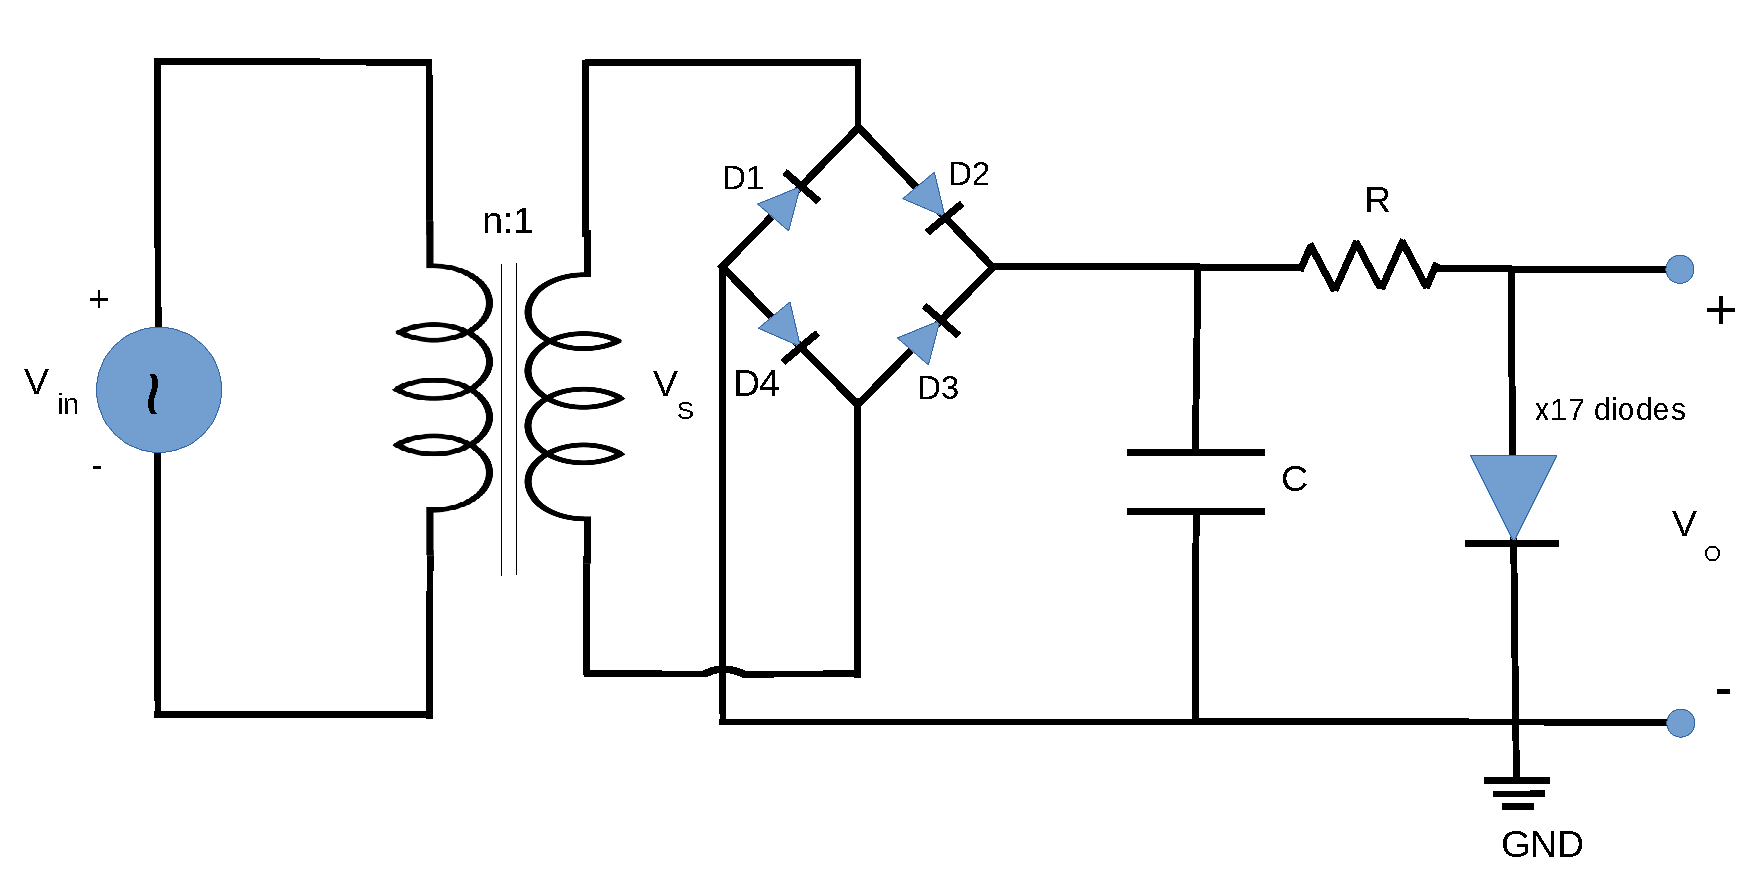
\includegraphics[scale=0.4]{lab3.pdf}
    \caption{Circuit analysed.}
    \label{fig:rc}
\end{figure}

The circuit is composed of several parts. The first one is a
transformer with a ratio of 1:n loops with the goal
of reducing the input's voltage by a factor of n.
Then we can find the remaining parts of the circuit: the envelope detector
and the voltage regulator.
Following the transformer is a full-wave bridge rectifier
composed of 4 diodes as shown.
In addition to the bridge rectifier, in the envelope detector we basically decided to insert a
capacitor with the objective of smoothing the "ripple", which is the residual
periodic variation of the DC voltage which has been derived from the AC source.
Lastly, in the voltage regulator we have a resistor in series with 18 diodes.


The way the full wave rectifier works is straightforward. The goal is to
simply transform a sinusoidal signal that can assume positive and negative values to only positive values.
We will simplify the circuit to a AC voltage source with the bridge rectifier and a load resistor as shown in figure \ref{fig:rc2} to explain.

When the input wave is positive, the route that the current takes is the following:
\begin{figure}[h] \centering
    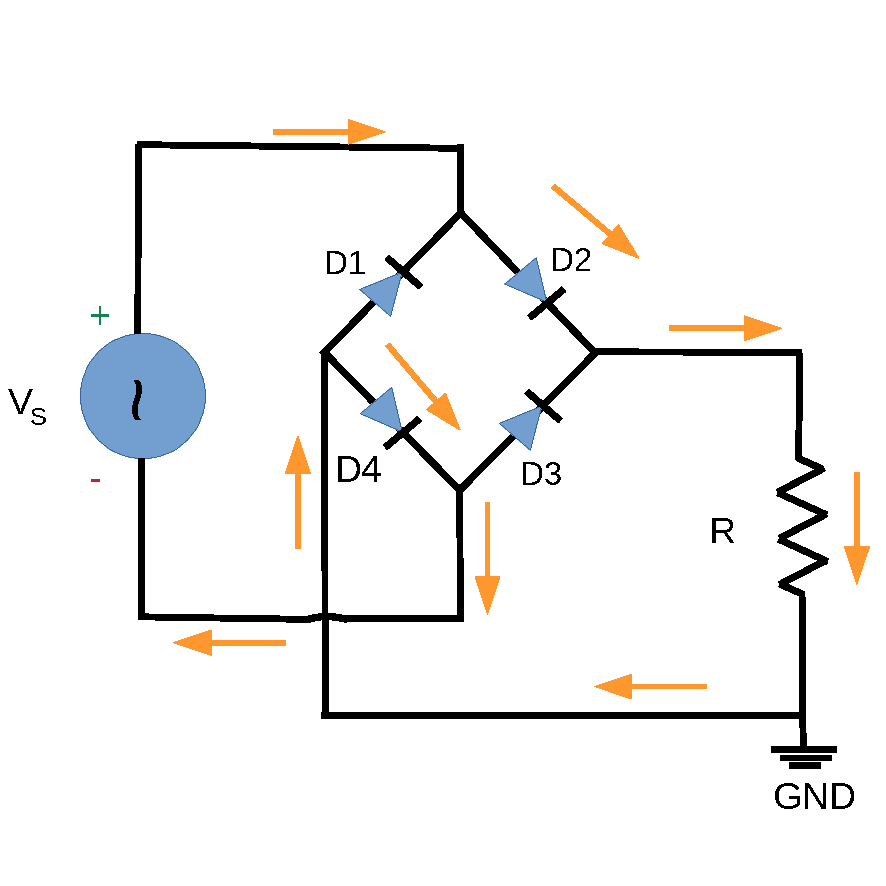
\includegraphics[scale=0.4]{lab3 _positive.pdf}
    \caption{Positive half.}
    \label{fig:rc2}
\end{figure}

This is because the diode D1 is in reversed bias and therefore
current can't pass through it. On the other hand, the diode D2 is in forward bias
so the current will go that way.
After it has passed the resistor, the current goes through the diode D4.
The reason it won't go through D1 is because the voltage drop in this diode
is negative.

When the input wave is negative, the path taken by the current is surprising, the current still flows in the same direction at the resistor!
\begin{figure}[h] \centering
    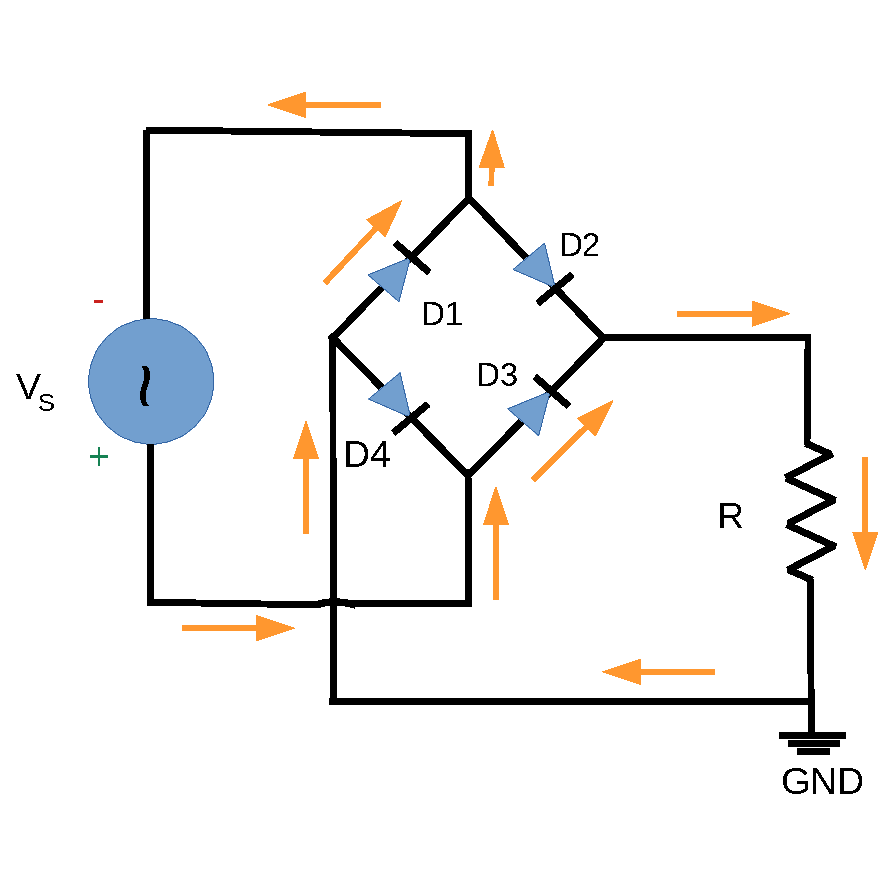
\includegraphics[scale=0.4]{lab3 _negative.pdf}
    \caption{Negative half.}
    \label{fig:rc3}
\end{figure}

The reasoning behind why the current goes though D3 and D1 is the same as
the reason why the current went through D2 and D4 in the positive half of the input wave as explained before.

In the end the objective we seeked was fullfilled as can be shown in the figure \ref{fig:rc4}.
\begin{figure}[h] \centering
    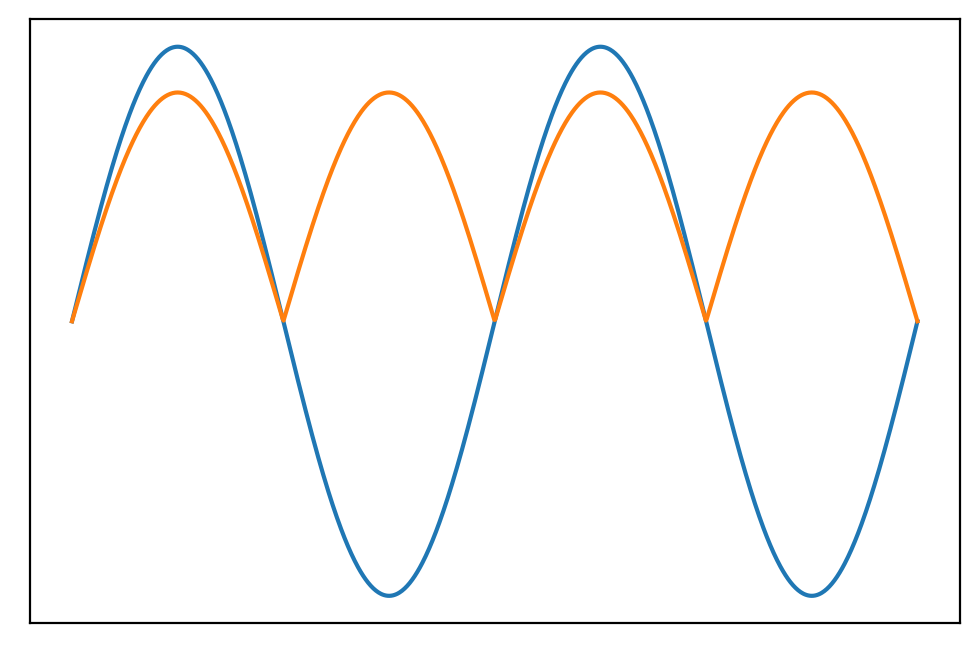
\includegraphics[scale=0.75]{rectwave.png}
    \caption{Wave rectified.}
    \label{fig:rc4}
\end{figure}

As we can see the voltage signal across the resistor (orange) has only positive values
meanwhile the input signal (blue) has both positive and negative values.

The capacitor we've put after the bridge rectifier in the figure \ref{fig:rc} allowed us to "smooth"
the voltage drop when the signal gets weaker. When the signal is stronger that the voltage limiter(in this case the resistor and diodes)
it allows the capacitor to charge so that, when the signal is not strong enough to support the voltage limiter, the capacitor
starts to discharge and in consequence the sub circuit containing the capacitor, resistor and diodes will still be
active while the rest of the circuit "stops". When the signal gets strong again, the capacitor charges again and this whole process repeats again.
\begin{figure}[h] \centering
    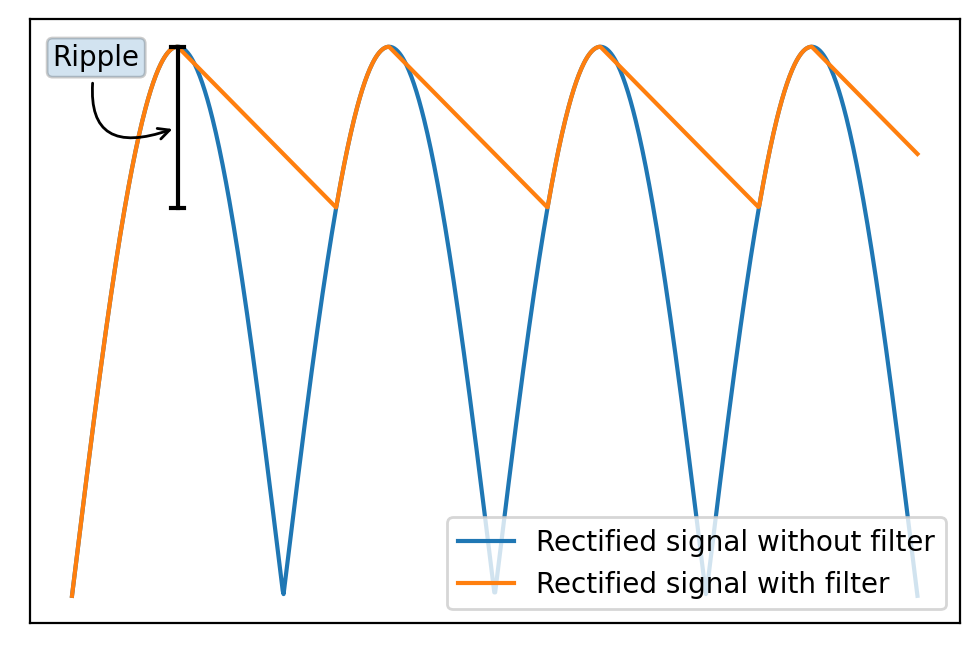
\includegraphics[scale=0.75]{filter.png}
    \caption{Wave rectified.}
    \label{fig:rc5}
\end{figure}

As we can see in figure \ref{fig:rc5} when the signal starts to drop the capacitor starts to discharge to provide
sufficient voltage for the circuit resistor-diode, that is why the slope demonstrate a "ripple" effect.

In section \ref{sec:analysis} we will give a theotherical analysis of the circuit chosen.
Hereinafter, in section \ref{sec:simulation}, we will simulate the same circuit using \emph{Ngspice}.
Finally, in section \ref{sec:conclusion}, we will compare the theotherical model to the simulation.

